\renewcommand{\lastmod}{14. November 2024}
\renewcommand{\chapterauthors}{Markus Lippitz}

\chapter{Quantentheorie des H-Atoms}


% \phet{Models_of_the_Hydrogen_Atom}

% \url{https://phet.colorado.edu/en/simulations/stern-gerlach}


%review : %https://phet.colorado.edu/sims/cheerpj/hydrogen-atom/latest/hydrogen-atom.html?simulation=hydrogen-atom


% 19. Hydrogen atom
% Sims: Models of the Hydrogen Atom, Rutherford Scattering (also falstad.com/qmatom)
% • It is extremely important in this section to relate the Schrodinger model of the atom back to
% the discussion of models of the atom earlier in the course (section 8), and show how this is the
% next step in the progression of models. Otherwise, students are likely to view this section as
% just one more example of a solution of the Schrodinger equation and not realize that we are
% actually talking about another model of the atom.
% • We have a homework in which we ask students to work through the simulations and explain
% the reasons for and limitations of each models. It’s amazing how difficult this is for students.


\section{Überblick}

In diesem Kapitel knüpfen wir an die Beschreibung der Atommodelle in Kapitel 2 an und führen das quantenmechanische Modell des Wasserstoffatoms ein. Die Lösung der dreidimensionalen Schrödingergleichung eines Elektrons im kugelsymmetrischen Coulomb-Potential liefert die gleichen Energien wie das Bohr'sche Modell, da sie mit dem Experiment übereinstimmen müssen. Außerdem findet man eine Quantisierung des Drehimpulses, wie sie auch von Bohr vorgeschlagen wurde, allerdings mit etwas anderen Werten.

Eine genauere Messung der Übergangslinien im Wasserstoffatom zeigt jedoch Abweichungen vom Bohr'schen Modell und damit auch von diesem einfachen quantenmechanischen Modell. Neben dem Coulomb-Potential gibt es noch weitere Beiträge zur potentiellen Energie des Elektrons. Zentral ist dabei der Spin des Elektrons, den wir zur Erklärung des Stern-Gerlach-Experiments einführen werden. Der Spin ähnelt einem Drehimpuls und ist mit einem magnetischen Moment verbunden. Ein Magnetfeld, das durch die Bahnbewegung entsteht, führt zu einem Energiebeitrag des magnetischen Moments.

Heute dient das Wasserstoffatom als Präzisionstest für unsere Modelle, deren Details hier den Rahmen sprengen würden. Derzeit gibt es jedoch keine Diskrepanz zwischen Theorie und Experiment.

Dieses und die beiden folgenden Kapitel sind in vielfältiger Weise miteinander verknüpft. An einigen Stellen muss ich daher den folgenden Kapiteln etwas vorgreifen. Die Reihenfolge ein Elektron -- viele Elektronen -- Magnetfeld ist nicht die einzig mögliche. In manchen Büchern ist die Reihenfolge anders. Ich beginne wieder mit \cite{Knight_physics}, um dann zu \cite{Demtröder_ep3} überzugehen. Gut lesbar finde ich immer noch \cite{Harris_moderne_Physik} und auch \cite{Heintze_WTA}.


\section{Schrödinger-Gleichung in 3 Dimensionen}
In der Quantenmechanik ist das Wasserstoffatom nur eine spezielle Form eines Potentialtopfs, nämlich ein dreidimensionaler Topf mit kugelsymmetrischem Potential, das durch das Coulombpotential gegeben ist. Das Potential hängt also nur vom Abstand $r$ zwischen Kern und Elektron ab, nicht von einer Richtung\sidenote{Ich verwende 'fette' Buchstaben wie $\br$ für Vektoren und 'dünne' Buchstaben wie $r$ für die Länge dieser Vektoren.}
\begin{equation}
    U(r) = - \frac{1}{4 \pi \epsilon_0} \, \frac{e^2}{r}
\end{equation}
weil sowohl Kern als auch Elektron jeweils die Ladung $\pm e$ tragen.

Im letzten Kapitel hatte ich die Schrödingergleichung in einer Dimension $x$ geschrieben, hier nun in 3 Dimensionen, ganz analog dazu
\begin{equation}
    - \frac{\hbar^2}{2m} \,\nabla^2 \, \Psi(\br) + \left[ U(\br) - E \right] \Psi(\br) = 0 \quad .
    \label{eq:5_SG_3d}
  \end{equation}
mit dem Quadrat des Nabla-Operators $\nabla^2$ als Abkürzung für
\begin{equation}
    \nabla^2 = \frac{\partial^2}{\partial x^2 } + \frac{\partial^2}{\partial y^2 } + 
    \frac{\partial^2}{\partial z^2 } 
\end{equation}
d.h. die Summe der doppelten (partiellen) Ableitungen in den drei Raumrichtungen. Wie im letzten Kapitel werden wir das nie wirklich selbst ausrechnen, sondern uns nur die Lösung anschauen. Die Rechnung findet man in jedem Buch zur Quantenmechanik.

\section{Quantenzahlen des Wasserstoff-Atoms}

In einer Dimension haben wir im letzten Kapitel gesehen, dass die Beschränkung des Teilchens auf einen Raumbereich zur Quantisierung der Energie und damit zur Quantenzahl $n$ führt, mit der wir die möglichen Energiewerte durchnummeriert haben. Nur diese Energien waren möglich, nur diese Wellenfunktionen lösten die Schrödingergleichung. Das gleiche gilt in drei Dimensionen. Schränkt man das Teilchen in drei Raumrichtungen ein, so erhält man drei Quantisierungen. Drei verschiedene Größen können nur bestimmte quantisierte Werte annehmen, wenn die Schrödingergleichung für das kugelsymmetrische Coulombpotential gelöst werden soll. Dies sind
\begin{description}
    \item[Hauptquantenzahl] Die Zahl $n$, die die Energien durchnummeriert, wird nun Hauptquantenzahl genannt, da weitere Quantenzahlen hinzukommen. Die zugehörigen Eigenenergien sind
 \begin{equation}
E_n = - \frac{1}{n^2} \left( \frac{1}{4 \pi \epsilon_0} \, \frac{e^2}{2 a_B }\right) = - \frac{13.6 \, eV}{n^2} \quad \text{mit} \quad n = 1,2, 3 \dots        \label{eq:5_En_Bohr}
    \end{equation}
    mit dem Bohr-Radius $a_B = 4 \pi \epsilon_0 \hbar^2 / (m e^2) \approx 0.5$\AA. Das sind die gleichen Energien, die wir auch im Bohrmodell gefunden haben.

    \item[Drehimpuls-Quantenzahl] Der Bahndrehimpuls $\bl$ des Elektrons\sidenote{In diesem Kapitel gibt es nur ein Elektron und Drehimpuls und Spin haben kleine Buchstaben. Im nächsten Kapitel ist das anders.} ist in seiner Länge  quantisiert
    \begin{equation}
        | \bl | = \hbar \sqrt{l (l+1) }  \quad \text{mit} \quad l = 0, 1,2, \dots , n-1 \quad .
    \end{equation}
Diese Zahl $l$ wird (Bahn-)Drehimpuls-Quantenzahl genannt.

\item[Magnetische Quantenzahl] Die z-Komponente $l_z$ des Bahndrehimpulses $\bl$ ist ebenfalls quantisiert 
\begin{equation}
    l_z = m \hbar   \quad \text{mit} \quad m = -l, -l+1, \dots, 0, \dots, l-1, l \quad .
\end{equation}
Diese Zahl $m$ wird magnetische Quantenzahl genannt. Den Grund für diesen Namen sehen wir unten.

\end{description}
Jeder stationäre Zustand des Wasserstoffatoms ist also durch drei Zahlen $(n,l,m)$ definiert. Jede dieser Zahlen beschreibt eine physikalische Eigenschaft des Atoms, wobei die Energie im Wasserstoffatom nur von der Hauptquantenzahl $n$ abhängt.

In anderen Atomen und bei einer Erweiterung des Modells aufgrund der Relativitätstheorie (siehe unten) hat dann auch die Drehimpulsquantenzahl $l$ einen Einfluss auf die Energie. Man bezeichnet daher die Zustände der Elektronen in Atomen mit den beiden Zahlen $n$ und $l$ (nicht aber $m$). Dazu kodiert man die Drehimpuls-Quantenzahl als Buchstaben nach folgendem Schema
\begin{equation}
    l = 0, 1, 2, 3 \quad \text{ergibt Buchstaben \ \ s, p, d, f} \quad .
\end{equation}
Der Zustand $(n,l) = (1,0)$ wird 1s genannt. Der Zustand $(n,l) = (3,2)$ heißt 3d. Da die magnetische Quantenzahl $m$ insgesamt $2l+1$ Werte annehmen kann, ist der Zustand 3d 5-fach entartet, der Grundzustand 1s dagegen nicht.

 
\begin{marginfigure}
    \inputtikz{\currfiledir H_SG_energien}
    \caption{Eigenenergien im Wasserstoffatom. Die vertikale Energie-Skala ist maßstabsgerecht.}
    \label{fig:5_H_SG_energien}
\end{marginfigure}

Abbildung  \ref{fig:5_H_SG_energien} zeigt die möglichen Zustände (ohne $m$-Entartung). Die Bedingung $n > l$ führt zu dieser dreieckigen Anordnung. Alle Zustände mit gleichem $n$ haben die gleiche Energie. Die Zustände liegen mit zunehmender Hauptquantenzahl $n$ immer näher an der Ionisationsgrenze $E=0$. Die Abhängigkeit von $n$ ist genau wie beim Bohr-Modell.


\section{Quantisierung des Drehimpulses}

Wir müssen noch etwas genauer auf den Drehimpuls eingehen. Wir haben schon beim Bohrmodell gesehen, dass der Bahndrehimpuls quantisiert ist. Damals konnte er nur ganzzahlige Vielfache von $\hbar$ annehmen. Jetzt ist es ähnlich, nur die Werte sind etwas anders, nämlich wie oben
\begin{equation}
    |\bl| = \hbar \sqrt{l (l+1) } = 0, \sqrt{2} \hbar, \sqrt{6} \hbar, \sqrt{12} \hbar, \dots
\end{equation}
mit einer ganzen Zahl $l \ge 0$.

Dies ist die \emph{Länge} des Drehimpulsvektors $\bl$. Seine drei kartesischen Komponenten sind $l_x$, $l_y$ und $l_z$ und natürlich
\begin{equation}
    |\bl|^2 =l_x^2 + l_y^2+ l_z^2 \quad .
\end{equation} 
Jede der kartesischen Komponenten muss kleiner als die Länge sein, also 
\begin{equation}
    l_{x,y,z}^2 \le |\bl|^2 = \hbar^2 l (l+1)
\end{equation}
Die Besonderheit des Drehimpulses in der Quantenmechanik ist nun, dass eine beliebige Komponente $l_{x,y,z}$ und die Länge 
$|\bl|$ zusammen gleichzeitig ohne Unschärfe gemessen werden können. Über die beiden anderen Komponenten kann man dann aber nichts mehr sagen, außer dass sie zusammen die richtige Gesamtlänge ergeben müssen. Wenn man also $l$ und $l_z$ gemessen hat, kann man nur noch sagen
\begin{equation}
    l_x^2 + l_y^2 = |\bl|^2  - l_z^2 \label{eq:5_l_kreis}
\end{equation}
Die Aufteilung zwischen $l_x$ und $l_y$ ist jedoch nicht festgelegt. Man kann sie sich als einen Vektor $\bl$ vorstellen, dessen Spitze auf einem Kreis liegt, der durch Gl.  \ref{eq:5_l_kreis} beschrieben wird, oder als einen Vektor, der einen Kegel beschreibt. Da $l_z$ ebenfalls quantisiert ist, gibt es $2l+1$ solcher Kreise bzw. Kegel.

Unabhängig davon, welche der drei kartesischen Komponenten gemessen wird, sind die beiden anderen immer innerhalb der genannten Grenzen unbestimmt. Typischerweise legt man das Koordinatensystem so an, dass die gemessene Komponente $l_z$ ist. In der Quantenmechanik ist es auch unerheblich, ob man diese Komponente tatsächlich misst oder nur messen kann\sidenote{wie beim Elektron im Doppelspalt}. Wie wir weiter unten sehen werden, ist der Drehimpuls mit einem magnetischen Moment verbunden, dessen Orientierung im Magnetfeld einen Energiebeitrag liefert. Die Orientierung eines äußeren Magnetfeldes definiert also die Richtung der z-Koordinate. Daher wird die Quantenzahl $m$ von $l_z$ auch als magnetische Quantenzahl bezeichnet.


\begin{marginfigure}
    \inputtikz{\currfiledir vector3d}
    \caption{Skizze eines Drehimpulsvektors mit unbekannter xy-Komponente.}
\end{marginfigure}
    


Eine Konsequenz der Quantisierung von $|\bl|$ und $l_z$ ist, dass der Vektor $\bl$ niemals exakt in z-Richtung orientiert sein kann. Es kann nie $l_z = |\bl|$ sein, weil $l_z$ ein ganzzahliges Vielfaches von $\hbar$ ist, $|\bl|$ aber diesen $\sqrt{l(l+1)}$-Term hat, der immer etwas größer als $l$ ist. Nur im Grenzfall sehr großer $l$ (im Korrespondenzprinzip) ist eine reine z-Orientierung möglich.

Weiterhin ist bemerkenswert, dass das Elektron im Grundzustand, d.h. im Zustand 1s, also $n=1$ und $l=0$, einen Bahndrehimpuls von Null hat. Ein klassisches Teilchen würde sich in diesem Fall überhaupt nicht auf einer geschlossenen Bahn bewegen. Für das Elektron in der Quantenmechanik ist das aber kein Problem.

\begin{marginfigure}
    \inputtikz{\currfiledir vector2d}
    \caption{Mögliche Orientierung von  Drehimpuls-artiger Vektoren mit $l=1/2$ (links) und $l=2$ (rechts). Der Abstand der Hilfslinien beträgt $1/2 \hbar$ bzw. $1\hbar$.}
\end{marginfigure}

Es gibt nicht nur Vektoren, die einem klassischen Drehimpuls entsprechen, sondern auch anderen Größen, die sich sehr ähnlich einem Drehimpuls verhalten, wie beispielsweise der Spin des Elektrons oder des Kerns. Bahndrehimpulse haben immer ganzzahlige Quantenzahlen $l$,$m$, Spins können auch halbzahlig sein. Immer ist der Abstand zwischen benachbarten Quantenzahlen aber eins. 


\begin{table}
    \begin{tabular}{ll}
        Drehimpuls & $\bl$ \\
        Betrag & $|\bl| = \hbar \sqrt{l (l+1) }$ \\
        Quantenzahl & $l$ \\
        Operator & $\hat{l}$ \\
        Eigenwerte &  $\hat{l}^2 \,  \Psi =  \hbar^2 \, l (l +1 )\,  \Psi  =|\bl|^2 \, \Psi $\\ 
        & \\
        z-Komponente & $l_z = \hbar m_l$ \\
        Quantenzahl & $m_l$ mit $|m_l| \le l$ \\
        Operator & $\hat{l}_z$ \\
        Eigenwerte &  $\hat{l}_z\,  \Psi =  \hbar \, m \,  \Psi  = l_z \, \Psi $\\ 
    \end{tabular}
\caption{Zusammenfassung der Beschreibung drehimpulsartiger Größen wie $\bs$, $\bj$, $\bF$, $\bI$. Im Fall von $\bl$ wird oft $m_l$ als $m$ geschrieben, ansonsten aber $m_s$, $m_j$ etc.}
\end{table}


\section{Wellenfunktionen}

Die Wellenfunktion $\Psi$, die die Schrödingergleichung löst, lässt sich am einfachsten in sphärischen Koordinaten schreiben, also statt $x,y,z$ als Funktion von $r,  \theta, \phi$. Die Lösungen besteht aus   drei Teilen: die Normierung, der Radialanteil $R(r)$ und der Winkelanteil $Y(\theta, \phi)$, also 
\begin{equation}
    \Psi_{n,l,m} (r, \theta, \phi) = A_{n,m} \, R_{n,l}(r) \, Y_l^m (\theta, \phi) \quad .
\end{equation}
Die $R_{n,l}(r)$ sind dabei Laguerre-Polynome und die $Y_l^m(\theta, \phi)$ Kugelflächenfunktionen.
Die ersten Wellenfunktionen sind
\begin{align}
    n,l,m  & & A_{n,m}                      & &R_{n,l}(r) & & Y_l^m(\theta, \phi) \\
   1,0,0   && \frac{1}{\sqrt{\pi a_B^3}}    & &e^{-r / a_B} && \\
   %
    2,0,0  & & \frac{1}{4 \sqrt{2 \pi a_B^3}}   & & \left( 2 - \frac{r}{a_B}\right) e^{-r /2 a_B} && \\
    2,1,0  & & \frac{1}{4 \sqrt{2 \pi a_B^3}}   & & \frac{r}{a_B} e^{-r /2 a_B} && \cos \theta \\
    2,1,\pm 1  & & \frac{1}{8 \sqrt{\pi a_B^3}}   & & \frac{r}{a_B} e^{-r /2 a_B} && \sin \theta \, e^{\pm i \phi} 
    %
\end{align}
mit dem Bohr-Radius $a_B$
\begin{equation}
    a_B = \frac{4 \pi \epsilon_0 \hbar^2}{\mu m_e^2}
\end{equation}
und der reduzierten Masse $\mu$. Manchmal kombiniert man die komplexen Wellenfunktionen mit $m = \pm 1$  zu solchen, die rein real sind. 


\section{Darstellung von 3d-Wellenfunktionen}

Im letzten Kapitel haben wir die eindimensionale Wellenfunktion $\Psi(x)$ entweder direkt auf der x-Achse aufgetragen oder als Wahrscheinlichkeitsdichte $P(x) = |\Psi(x)|^2$ dargestellt. Im Eindimensionalen ist dies leicht möglich. Im Dreidimensionalen ordnet die Wahrscheinlichkeitsdichte jedem Punkt $\br$ im Raum einen Wert zu. Dies ist schwierig darzustellen. Zum einen ist Papier oder ein Bildschirm immer nur zweidimensional. Zum anderen verdecken 'vordere' Werte die dahinter liegenden, wenn der Wert z.B. als Farbe kodiert ist.

\begin{marginfigure}
    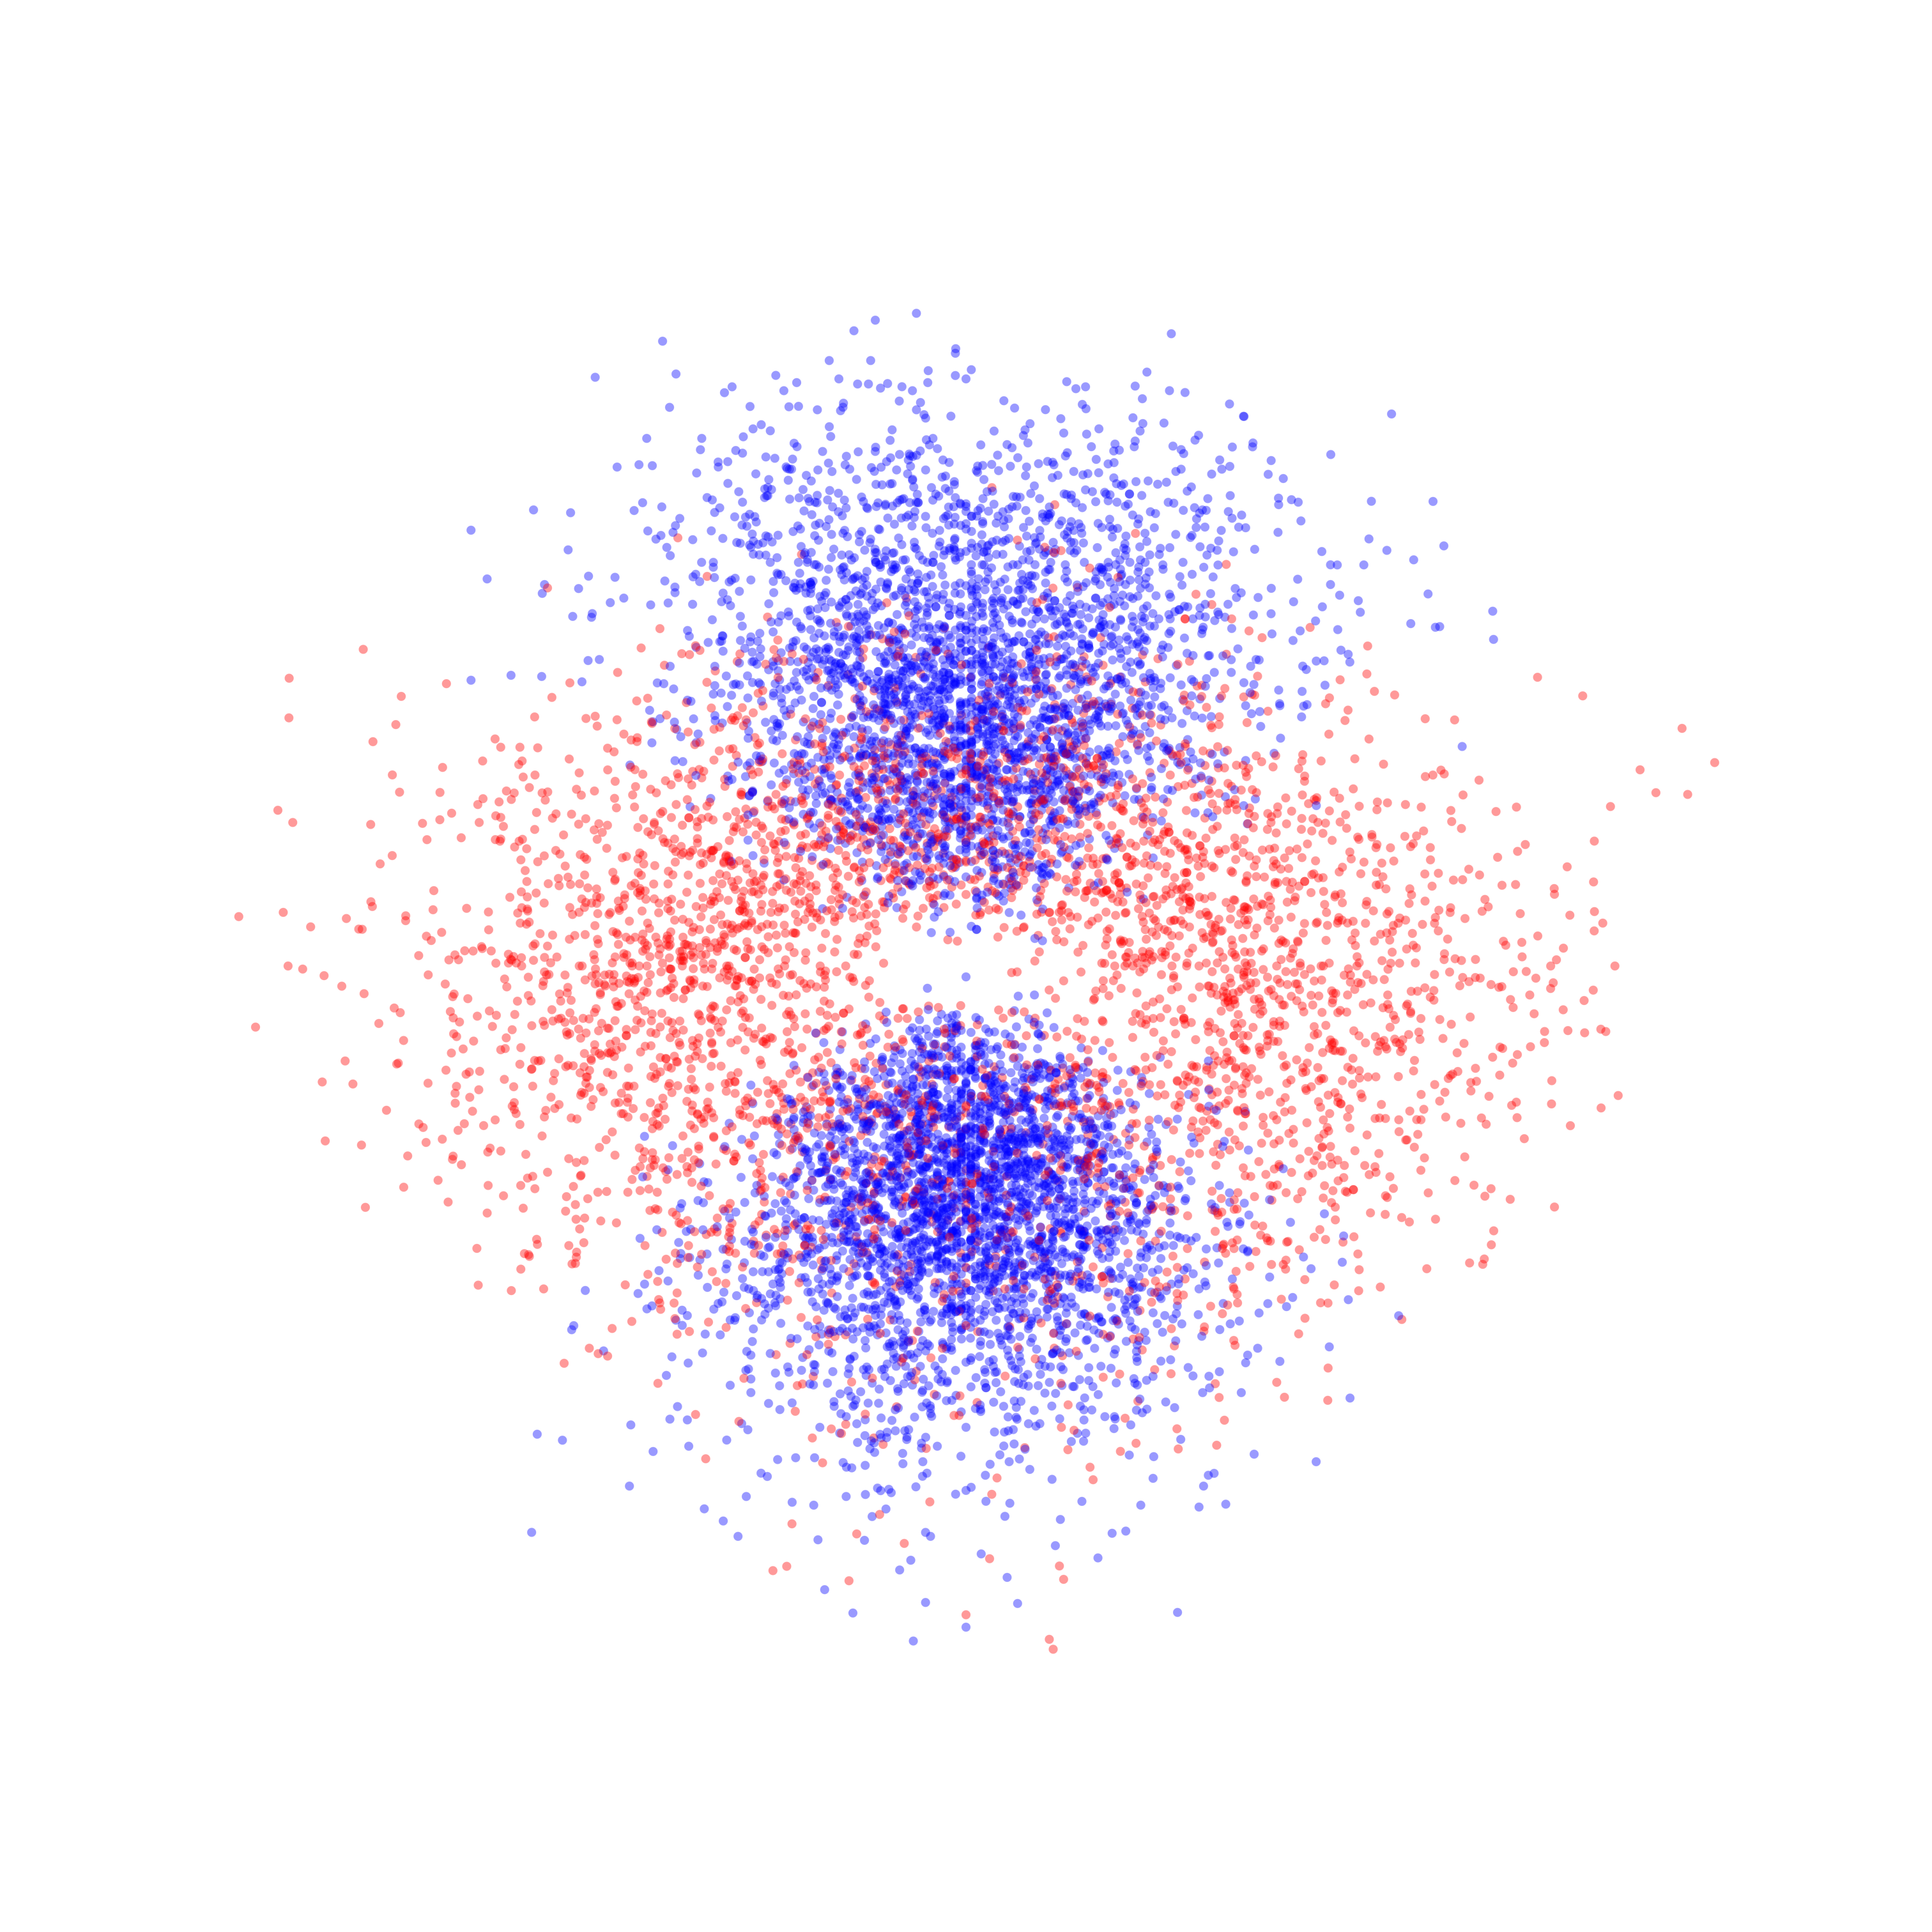
\includegraphics[width=40mm]{\currfiledir pluto/scatter_WF.png}
    \caption{Wellenfunktion eines 3d-Zustandes als Punktwolke simulierter Detektionsereignisse. Das Vorzeichen der Wellenfunktion ergibt die Farbe des Punktes.}
\end{marginfigure}


Es gibt verschiedene Möglichkeiten, die jedoch alle ihre Vor- und Nachteile haben (Die folgenden Abbildungen zeigen Beispiele):
\begin{description}
    \item[Punktwolke] Man kann die Detektion des Elektrons an verschiedenen Orten simulieren und in eine Punktwolke eintragen. Je näher die Punkte beieinander liegen, desto höher ist die Wahrscheinlichkeitsdichte. Die Gesamtzahl der Punkte muss klein gehalten werden, damit die Wolke noch einigermaßen durchsichtig ist. Am Computer kann man die Wolke drehen, um einen dreidimensionalen Eindruck zu erhalten.
    \item[Iso-Flächen] Man kann Flächen $P(\br) = |\Psi(\br)|^2 = const.$ zeichnen, ähnlich den Isobaren im Wetterbericht. Wenn die Konstante gut gewählt ist, erhält man eine Vorstellung von der Wellenfunktion. Diese kann dreidimensional dargestellt oder mit einer Ebene geschnitten werden.
    \item[Schnitte] Man kann $P(x,y)$ farbkodiert auf einer Ebene darstellen. Die Ebene enthält fast immer den Atomkern. Manchmal ist es hilfreich, eine zweite Ebene senkrecht dazu darzustellen.
    \item[Radiananteil] Anstatt zu fragen, wie groß die Wahrscheinlichkeit ist, das Elektron am Ort $\br$ zu finden, kann man fragen, wie groß die Wahrscheinlichkeit ist, es im Abstand $r$ vom Kern zu finden. Dies ist die \emph{radiale Wahrscheinlichkeitsdichte} $P_r(r)$.
    \begin{equation}
        P_r(r) = \iint P(r, \theta, \phi) \, d\theta d\phi = 4 \pi r^2 |R_{n,l}(r)|^2 \quad .
    \end{equation}
    Der Term $4 \pi r^2$ berücksichtigt, dass mit zunehmendem Radius $r$ die Anzahl der Möglichkeiten und also das Volumen der Kugelschale zunimmt.
\end{description}

\begin{figure}[tb]
    \inputtikz{\currfiledir WF_3d_panel}
    \caption{Iso-Flächen der Wellenfunktionen $\Psi(\br)$. Angegeben sind die Quantenzahlen $(n,l,m,)$. Die Farbe kodiert das Vorzeichen. Die Größe ist willkürlich skaliert.}
\end{figure}

Die verschiedenen Darstellungen scheinen sich zu widersprechen. Alle s-Wellenfunktionen (also $l=0$) haben ein Maximum bei $P(\br = 0)$, aber eine Nullstelle bei $P_r(r=0)$. Der wahrscheinlichste Ort für ein Elektron ist daher der Kern. Gleichzeitig ist der wahrscheinlichste Abstand vom Kern weit von Null entfernt.  Dies sind jedoch zwei verschiedene Fragen.  Für große Abstände gibt es viel mehr Möglichkeiten auf der Kugeloberfläche. Jede dieser Möglichkeiten ist für sich jedoch unwahrscheinlicher als der Ort auf dem Kern.


\begin{figure}[tb]
    \inputtikz{\currfiledir WF_P_2d_panel}
    \caption{Schnitt der Wellenfunktion $\Psi(\br)$ und der Wahrscheinlichkeitsdichte $P(\br)$ in der xy-Ebene. Die Längen sind mit $1/n^2$ skaliert, die Wellenfunktionen mit $1/n^3$. Die Farbe kodiert das Vorzeichen.}
\end{figure}



\begin{marginfigure}
    \inputtikz{\currfiledir radial_P}
    \caption{Radiale Aufenthaltswahrscheinlichkeiten  $P_r(r)$ für $n=1,2,3$.}
\end{marginfigure}

Betrachtet man die radiale Aufenthaltswahrscheinlichkeit $P_r(r)$, so stellt man fest, dass die Wellenfunktionen mit dem größten $l$ bei gegebenen $n$, also 1s, 2p, 3d usw., ihre Maxima bei den von Bohr erwarteten Radien, also $1 a_B$, $4 a_B$ und $9 a_B$ haben. Die anderen Wellenfunktionen liegen mit einer gewissen Wahrscheinlichkeit weiter außen. Dies ist eine weitere Konsequenz des Korrespondenzprinzips. Für große Quantenzahlen $l$ werden die Elektronen immer klassischer, die Bahnen immer kreisförmiger, immer näher am Bohrschen Modell. Bei kleinen Bahndrehimpulsen ist die Bahn nicht mehr so kreisförmig, bis hin zur s-Wellenfunktion ohne Bahndrehimpuls.

Die Schrödingergleichung gibt also die von Bohr postulierten Bahnen wieder, aber nur als Maximum der Wahrscheinlichkeit, den Bahnradius zu messen. Mit einer gewissen Wahrscheinlichkeit sind auch andere Bahnradien möglich. Noch einmal: In der Quantenmechanik bewegt sich das Elektron nicht auf einer geschlossenen Bahn. Allerdings entspricht die Wahrscheinlichkeitsdichte, das Elektron in einem bestimmten Abstand vom Kern zu finden, dem klassischen Bahnmodell.



\section{Relativistische Korrekturen}


Wenn man die Energien der Zustände sehr genau bestimmt, z.B. durch optische Spektroskopie der Übergänge zwischen ihnen, findet man leichte Abweichungen von den in Gleichung \ref{eq:5_En_Bohr} beschriebenen Energien. Einige Beiträge hierzu sollen hier kurz erwähnt werden. Details finden sich in \cite{Demtröder_ep3}.
\begin{description}
    \item[Relativistische Massenzunahme]  Eigentlich müsste man die Energien relativistisch berechnen, d.h. die relativistische Massenzunahme berücksichtigen. Wenn man dies tut, findet man in niedrigster Ordnung einen Term, der in etwa mit $v/c$, dem Verhältnis der Elektronengeschwindigkeit zur Lichtgeschwindigkeit, übereinstimmt. Dies ist die \emph{Sommerfeld'sche Feinstrukturkonstante} $\alpha$
\begin{equation}
    \alpha = \frac{e^2}{4 \pi \epsilon_0 \hbar c} \approx \frac{1}{137} \approx \frac{v}{c}
\end{equation}
Sie führt zu einer relativen Verschiebung der Energien der Zustände um etwa $10^{-4}$, die im Detail von den Quantenzahlen $n$ und $l$ abhängt, so dass die Entartung von Zuständen mit gleichem $l$ aufgehoben wird.\sidenote{Diese Korrektur hätte man auch schon im Bohr-Modell anwenden können, was das Bohr-Sommerfeld-Modell ergibt.} 

    \item[Positionsunschärfe] Die momentane Position des Elektrons kann nicht beliebig genau bestimmt werden. Daher ist auch der Wert des Coulombpotentials am Ort des Elektrons nicht genau bekannt, sondern muss über einen bestimmten Raumbereich gemittelt werden. Dies ergibt eine Verschiebung der Energien um den \emph{Darwin Term}, der von der Aufenthaltswahrscheinlichkeit des Elektrons am Kern abhängt, also von $|\Psi(0)|^2$. Hierdurch werden die Energien der s-Wellenfunktionen noch einmal verschoben.
    
    \item[Elektronen-Spin]  Schließlich gibt es noch den Elektronenspin, eine weitere intrinsische Eigenschaft des Elektrons wie Masse und Ladung, die mit einem magnetischen Moment verbunden ist. Der Spin wird im folgenden von Bedeutung sein und verdient eine nähere Betrachtung.
\end{description}




\section{Das Stern-Gerlach Experiment}

Ich greife hier dem Kapitel über Atome im Magnetfeld etwas vor.
Die Bahnbewegung des Elektrons kann als Strom aufgefasst werden und ist mit einem magnetischen Moment $\bmu$ verbunden.
\begin{equation}
    \bmu = - \frac{e}{2 m_e} \,  \bl \quad .
\end{equation}
Die Messung des magnetischen Moments gibt also Auskunft über den Bahndrehimpuls $\bl$.
Um 1922 wollten Otto Stern und Walter Gerlach deshalb das magnetische Moment von Atomen messen und damit den Bahndrehimpuls bestimmen. Rückblickend haben sie damit den Spin des Elektrons gefunden.\footcite{SEP_Stern_gerlach}


Die potentielle Energie eines magnetischen Moments in einem magnetischen Feld beträgt
\begin{equation}
    U_B = - \bmu \cdot \bB \quad .
\end{equation}
Daher wirkt eine Kraft $\bF_B$
\begin{equation}
    \bF_B = - \text{grad} ( U_B ) =  \text{grad} (\bmu \cdot \bB ) = \mu_z \cdot \frac{\partial B}{\partial z} \quad .
\end{equation}
Im letzten Schritt wurde die übliche Annahme getroffen, dass das Magnetfeld in z-Richtung orientiert ist. Eine räumliche Änderung (in z-Richtung) des Magnetfeldes bewirkt somit eine Kraft auf einen magnetischen Dipol, die proportional zur z-Komponente des Dipols ist.

\begin{marginfigure} 
    \inputtikz{\currfiledir SG_setup}
    \caption{Stern-Gerlach Versuch. Ein Strahl von Silberatomen wird im inhomogenen Magnetfeld aufgespaltenen.}
\end{marginfigure}

Dies kann man sich auch anschaulich vorstellen, wenn man sich den magnetischen Dipol als Stabmagnet vorstellt. Befindet sich der Nordpol des Magneten an einer größeren z-Koordinate, so ist die Kraft auf ihn größer als die Kraft auf den Südpol, weil das Feld mit z stärker wird. Daraus ergibt sich eine Nettokraft in positiver z-Richtung. 

Im Experiment erzeugten Stern und Glerach einen Gradienten im Magnetfeld, indem sie einen Polschuh des Magneten kleiner machten als den anderen, so dass dort die Feldlinien enger zusammenliefen und das Feld stärker war. Durch ein solches inhomogenes Magnetfeld ließen sie  Silberatome laufen. 
Stern und Gerlach wählten Silber, weil sich hier alle Elektronen bis auf eines in voll besetzten Schalen befinden, wie wir im nächsten Kapitel sehen werden. Tatsächlich bleibt nur der Einfluss dieses letzten Elektrons übrig, der Rest hebt sich gegenseitig auf. Damals dachte man, dass dieses letzte Elektron die Quantenzahl $l=1$ besitzt.
 Silber wird also in einem Ofen erhitzt und der austretende Silberdampf durch Blenden kollimiert, so dass ein atomarer Silberstrahl entsteht. Dieser wird in dem Magnetfeld abgelenkt und auf einer Glasplatte detektiert.

Bei ausgeschaltetem Magneten ergibt sich eine horizontale Linie, die der horizontalen Blende entspricht. Bei eingeschaltetem Magneten werden die Atome entsprechend ihrem magnetischen Moment vertikal abgelenkt.
 Für ein Elektron im Zustand $l=1$ erwartet man 3 Linien, für jede der  magnetischen Quantenzahlen $m=-1, 0, +1$. Ein solches Ergebnis würde bedeuten, dass der Bahndrehimpuls quantisiert ist.

\section{Der Spin}

Stern und Gerlach fanden nicht drei, sondern nur zwei Linien und entdeckten damit den Elektronenspin, bevor dieses Konzept überhaupt erfunden wurde.\sidenote{Details siehe \cite{SEP_Stern_gerlach}} Heute wissen wir, dass sich das relevante Elektron im Silberatom im Zustand $l=0$ befindet, der Bahndrehimpuls selbst also keine Aufspaltung liefert. Woher stammen dann die beiden beobachteten Linien?

Ein Elektron hat eine Masse und eine Ladung, die für die Gravitationskraft und die Coulombkraft relevant sind. Es hat sich herausgestellt, dass ein Elektron noch eine weitere Eigenschaft besitzt, ein magnetisches Moment. Dieses innere magnetische Moment des Elektrons nennt man Spin.  Ein geladener Ball, der sich um sich selbst dreht, hätte solch ein magnetisches Moment, das mit dieser Drehung verbunden ist. Das Elektron dreht sich aber nicht wirklich, sondern nur in
unserer Vorstellung. Der Spin-Drehimpuls des Elektrons ist aber wirklich vorhanden, wie das Einstein--de Haas--Experiment zeigt, das wir im Kapitel über Atome im Magnetfeld besprechen werden.

Für Elektronen ist der Spin $\bs$ mit
\begin{equation}
    | \bs | = \hbar \sqrt{s (s+1)} \quad \text{mit} \quad s = \frac{1}{2} \quad .
\end{equation}
Auch andere quantenmechanische Teilchen besitzen diesen eingebauten Drehimpuls, den Spin, der dort auch andere Längen $ | \bs |$ und Quantenzahlen $s$ annehmen kann.

Analog zum Bahndrehimpuls ist auch die Orientierung des Spins quantisiert. Die Spanne der möglichen Werte ist wiederum $\hbar$, so dass nur die Werte 
\begin{equation}
   s_z = m_s \hbar \quad \text{mit} \quad m_s = \pm \frac{1}{2}
\end{equation}
möglich sind. Der Zustand $m_s = + 1/2$ mit $s_z = \hbar /2$ wird als 'spin up' bezeichnet, der andere als 'spin down', was manchmal durch $\uparrow$ und $\downarrow$ symbolisiert wird.\sidenote{Wie oben kann der Spin nicht vollständig in z-Richtung zeigen}.


\section{Spin-Bahn-Kopplung}

Das magnetische Moment $\bmu$, das mit dem Spin $\bs$ des Elektrons verbunden ist, führt zu einem Energiebeitrag in der Schrödinger-Gleichung, der als \emph{Spin-Bahn-Kopplung} bezeichnet wird. Dazu ändern wir die Perspektive und setzen uns auf das Elektron. Dann umkreist der Kern das Elektron. Der Kern ist positiv geladen und seine Kreisbewegung entspricht einem Kreisstrom, der mit einem Magnetfeld $\bB \propto \bl$ verbunden ist. Dieses Feld trägt zur potentiellen Energie des Elektrons bei
\begin{equation}
    U_{ls} = - \bmu \cdot \bB = \cdots = \frac{e^2 \mu_0}{8 \pi m_e^2 r^3} \, \bl \cdot \bs
\end{equation}
In der Quantenmechanik muss der Erwartungswert $\braket{U_{ls}}$ verwendet werden, also
\begin{equation}
    E_{ls} = \braket{U_{ls}} = \frac{e^2 \mu_0}{8 \pi m_e^2 r^3} \, \braket{\bl \cdot \bs}
    = \frac{a}{\hbar^2} \, l \, s \, \cos \phi
\end{equation}
mit dem Winkel $\phi$ zwischen den Vektoren $\bs$ und $\bl$ und der Spin-Bahn-Kopplungskonstante $a$
\begin{equation}
    a = \frac{e^2 \mu_0 \hbar^2}{8 \pi m_e^2 r^3} \quad . 
\end{equation}

Man beschreibt nun den Term $l \, s \, \cos \phi$ bzw. den Winkel $\phi$ zwischen den Vektoren $\bs$ und $\bl$ über die Vektorsumme $\bj = \bl + \bs$ . Die Vektoren $\bs$, $\bl$ und $\bj$ bilden ein Dreieck, für dessen Kantenlänge gilt
der Kosinussatz
\begin{equation}
    |\bj|^2 =   |\bs|^2 +   |\bl|^2  - 2 \, l \, s \, \cos (\pi - \phi) \quad .
\end{equation}
Für Vektoren gilt allgemein $|\bj|^2  = \bj \cdot \bj = \bj^2$, also 
\begin{equation}
    \bj^2 =   \bs^2 +   \bl^2  + 2  \bl \cdot \bs
\end{equation}
also
\begin{equation}
    \bl \cdot \bs = \frac{1}{2} \left[ \bj^2 -  \bl^2 -   \bs^2   \right]
    = \frac{\hbar^2}{2} \left[ j(j+1) - l(l+1) - s(s+1) \right]
\end{equation}
und somit schließlich
\begin{equation}
    E_{ls}     = \frac{a}{2}  \left[ j(j+1) - l(l+1) - s(s+1) \right] \quad . 
    \label{eq:5_FS_ls}
\end{equation}

Welche Werte kann $\bj$ bzw. seine Quantenzahl $j$ annehmen? Wir haben $\bj$ als Vektorsumme von $\bl$ und $\bs$ eingeführt. Vom Spin $\bs$ wissen wir, dass seine Länge immer durch $s=1/2$ beschrieben ist und die Richtung nur zwei Werte annehmen kann, up und down. Damit ist \emph{hier noch} $j = l \pm 1/2$. Für Atome mit mehr als einem Elektron wird dies anders sein, wie wir im nächsten Kapitel sehen werden.


\section{Alle relativistischen Korrekturen zusammen}

\begin{marginfigure}[-20mm]
    \inputtikz{\currfiledir H_sl_energien}
    \caption{Die Spin-Bahn-Kopplung führt zu einer Aufspaltung nach $j$. Grau eingezeichnet sind die Bohr-Niveaus. In der Darstellung ändert sich die Energie-Skalierung mit $n$.}
    \label{fig:5_H_sl_energien}
\end{marginfigure} 

Nimmt man alle drei relativistischen Korrekturen zusammen, die Massenzunahme, die Positionsunschärfe und die Spin-Bahn-Kopplung, so erhält man im Wasserstoffatom Eigenenergien, die nur noch von $n$ und $j$, aber nicht mehr von $l$ abhängen. ($s$ ist ohnehin immer $1/2$, nur die Richtung des Spins $m_s$ ist relevant).
\begin{equation}
    E_{n,j} = E_n \left[ 1 + \frac{\alpha^2}{n} \left( \frac{1}{j + 1/2} - \frac{3}{4n} \right) \right]
\end{equation}
Wir ergänzen die Bezeichnung der Zustände durch ein tiefergestelltes $j$. Die Zustände 2s$_{1/2}$ und 2p$_{1/2}$ haben also die selbe Energie, ebenso  3p$_{3/2}$ und 3d$_{3/2}$. Abbildung \ref{fig:5_H_sl_energien} skizziert dies.




\section{Kernspin}

Auch der Atomkern besitzt einen Spin $\bI$ und damit ein magnetisches Moment. Dieses magnetische Moment besitzt eine potentielle Energie im Magnetfeld, das durch die Bahn des Elektrons am Ort des Kerns erzeugt wird. Dies ist völlig analog zur Spin-Bahn-Kopplung und wird durch einen Gesamtdrehimpuls $\bF = \bj + \bI$ beschrieben. Sie liefert eine Hyperfeinstruktur analog zu Gl. \ref{eq:5_FS_ls}.
\begin{equation}
    E_{HFS}     = \frac{A}{2}  \left[ F(F+1) - j(j+1) - I(I+1) \right] \quad . 
\end{equation}
mit der Hyperfeinstrukturkonstanten $A$.


\section{Der Messprozess in der Quantenmechanik}

Ich wollte oben beim Spin den Bogen bis zur Spin-Bahn-Kopplung nicht zu lang werden lassen und füge deshalb hier einen Aspekt hinzu. Beim Stern-Gerlach-Experiment lohnt es sich, über den quantenmechanischen Messvorgang nachzudenken. 

Eine quantenmechanische Messung verändert die Wellenfunktion. Sei $\hat{Q}$ ein Operator, der die Quantenzahl $Q$ bestimmt, die die Werte $Q=1,2,3$ usw. annehmen kann. Die zugehörigen Eigenfunktionen $\Psi_Q$ bilden ein Orthonormalsystem. In diesem Eigenfunktionen kann dann eine allgemeine Wellenfunktion $\Psi$ entwickelt werden. Vor der Messung ist die Wellenfunktion
\begin{equation}
    \Psi_{vorher} = \sum_Q a_Q  \, \Psi_Q \quad \text{mit} \quad \sum_Q |a_Q|^2 = 1
\end{equation}
Die Wahrscheinlichkeit, den Wert $Q=1$ zu messen, ist dann $|a_1|^2$. Direkt nach der Messung ist dann aber die Wellenfunktion in dem zugehörigen Eigenzustand des Operators, also 
\begin{equation}
    \Psi_{nachher} = \Psi_1
\end{equation}
Wenn ich direkt zweimal hintereinander messe, erhalte ich den gleichen Wert. (Bei Operatoren mit koninuierlichen Eigenwerten, wie z.B. der Position, ist es komplizierter, da ich die Position nur mit einer gewissen Genauigkeit wirklich kenne.)


Im Stern-Gerlach-Experiment bestimmen wir den Wert von $j_z$, also die z-Komponente des Gesamtdrehimpulses $\bj$. Wenn man nun einen der aufgespaltenen Teilstrahlen abtrennt, kennt man $j_z$ der Atome in diesem Strahl. Eine erneute Messung von $j_z$ in einem zweiten Stern-Gerlach-Aufbau liefert daher den gleichen Wert und keine weitere Aufspaltung des Strahls. Das oben beschriebene Stern-Gerlach-Experiment setzt also voraus, dass Atome mit einem unbestimmten $j_z$ aus dem Ofen austreten.


Man kann aber auch das zweite Stern-Gerlach-Experiment drehen und z.B. $j_x$ messen. Wenn $j_z$ aus der ersten Messung bekannt ist, dann ist $j_x$ maximal unscharf und man erhält wieder eine Aufspaltung des Strahls in die $2j+1$ Möglichkeiten von $j_x$.

Diese Messung von $j_x$ bei der zweiten Stern-Gerlach-Aperatur verändert jedoch die Wellenfunktion. Nach der zweiten Messung befindet sich das Atom in einer Eigenfunktion des $j_x$-Operators, die keine Eigenfunktion des $j_z$-Operators ist. In einer anschließenden dritten Stern-Gerlach-Messung, die wieder $j_z$ misst, wird man wieder eine Aufspaltung finden, auch wenn man nach der ersten $j_z$-Messung nur die Atome selektiert hat, die einem einzigen Wert von $j_uz$ entsprechen!


\section{Zusammenfassung}

\textit{Schreiben Sie hier ihre persönliche Zusammenfassung des Kapitels auf. Konzentrieren Sie sich auf die wichtigsten Aspekte.}

\vspace*{10cm}



%--------------------
\printbibliography[segment=\therefsegment,heading=subbibliography]
